%! TEX root = ../aminhash.tex

\section{Evaluation by Experimentation}\label{sec:evaluation}

In this section, we show our proposed estimators lead to improved performance on maximum
Jaccard similarity search on real datasets.

. First, we fix the quantization
mechanism and compare traditional reconstruction
loss with our proposed loss to show that score-aware
loss leads to better retrieval performance and more accurate estimation of maximum inner product values.
Next, we compare in fixed-bit-rate settings against
QUIPS and LSQ, which are the current state-of-the art for many MIPS tasks. Finally, we analyze the
end-to-end MIPS retrieval performance of our algorithm in terms of its speed-recall trade-off in a
standardized hardware environment. We used the
benchmark setup from ann-benchmarks.com, which
provides 11 competitive baselines with pre-tuned parameters. We plot each algorithm’s speed-recall curve
and show ours achieves the state-of-the-art.

Mention stuff about
Use of Stirling's approximation.
Use of Newton's method.

\subsection{Recall vs Memory usage}

We focus on the measure recall@10, which means how often the estimated top 10 most similar sets contain the true most similar set.
If the searcher wants to obtain the true nearest set, they can use the estimation as a fast first scan over the data, and then compute the true similarities between the query and the 10 candidates.

We are interested in how the number of hash functions / hash values per stored set trades with the recall.
The number of such values is directly proportional to the memory required to store the dataset.
%We measure memory in the number of independent hash functions we need to store values from.
\footnote{Each value can be stored in a word, and it is possible to compress them further, usually down to around a byte without loss of accuracy.}

The following shows the effect on recall@10 with 10,000 queries:

These results use the minhash estimator as the initial guess.
An alternative is to estimate $v$ as $by/K$, since $Eb=v/y$.
However that appears to be worse, giving recall 1@10 of 0.1718 at newton=1 and $K=30$.
With more newton steps, however, the recall "recovers" to 0.1889 at newton=8.
($n=2$ and $n=4$ gives recall 0.1754 and 0.1826 respectively.)

%Some timing data:
%Tid for -K 100 --newton 1
%Time preparing: t1=2813.205824613571, Time searching: t2=5754.812134742737
%Tid for -K 100 --newton 2
%Time preparing: t1=2768.65847158432, Time searching: t2=5648.562669038773
%Tid for -K 100 --newton 4
%Time preparing: t1=2715.9863698482513, Time searching: t2=5616.8901562690735
%Tid for -K 100 --newton 8
%Time preparing: t1=2769.066630601883, Time searching: t2=6230.902306318283
%
%-K 1 --newton 8
%Time preparing: t1=31.681596994400024, Time searching: t2=765.3667838573456

The first table was wrong, because it didn't account for points with equal similarity.
The following table fixes that problem:
\begin{table}
\centering
 \begin{tabular}{|r| r r r r r|} 
 \hline
     \multicolumn{6}{|c|}{Recall@10 on the Netflix dataset} \\
 \hline
 K  & Classic & MLE & Minner & Minner 1N & Minner 8N \\
 \hline
    1 & 0.0033 & 0.0076 & \textbf{ 0.0099} & 0.0057 & 0.0063 \\
  10 & 0.0501 & 0.0396 & \textbf{ 0.0623} & 0.0506 & 0.0462 \\
  30 & 0.1474 & 0.1773 & \textbf{ 0.1914} & 0.1910 & 0.1862 \\
 100 & 0.3831 &      . & 0.4640 & 0.4870 & \textbf{ 0.4903} \\
 400 & 0.7510 &      . & 0.8054 & 0.8326 & \textbf{ 0.8338} \\
 500 & 0.7942 &      . & 0.8440 & 0.8660 & \textbf{ 0.8667} \\
  \hline
 \end{tabular}
 \caption{The Minner estimator is best at small $K$, but eventually the asymptotics kick in and the Maximum likelihood estimator overtakes. The MLE is very slow however, and one can get most of the benefits by applying a single iteration of Newton's method on top of the Minner Estimator.}
 \label{tab:netflix}
\end{table}

We can also test on the Flickr Dataset
\begin{table}
\centering
 \begin{tabular}{|r| r r r r r|} 
 \hline
     \multicolumn{6}{|c|}{Recall@10 on the Flickr dataset} \\
 \hline
 K  & Classic & MLE & Minner & Minner 1N & Minner 8N \\
 \hline
    1 & 0.2379 & 0.3410 & \textbf{ 0.3595} & 0.2806 & 0.2969 \\
   5 & 0.6256 & 0.5457 & \textbf{ 0.6688} & 0.5913 & 0.6138 \\
  10 & 0.7770 & 0.7155 & \textbf{ 0.8122} & 0.7327 & 0.7469 \\
  20 & 0.8657 & 0.8540 & \textbf{ 0.8963} & 0.8217 & 0.8352 \\
  30 & 0.9108 & 0.9080 & \textbf{ 0.9301} & 0.8597 & 0.8714 \\
  \hline
 \end{tabular}
 \caption{The Flickr dataset is much easier than the Netflix dataset and as such doesn't require as many MinHash values to obtain good recall. The Maximum likelihood estimator never overcomes its asymptotic disadvantage, but the Minner Estimator beats the Classic estimator by up to $51\%$ at $K=1$.}
 \label{tab:flickr}
\end{table}

%\subsection{Estimation: Hash functions vs Accuracy}
\subsection{Estimation: One way complexity of set similarity}
\label{sec:estimation}

TODO: Say something about \cref{fig:exp_variance}

We also perform some experiments on estimation.
While this is not the main focus of the paper, we note that the results are consistent with the variance computed for the MLE estimator.

\begin{figure}
   %\hspace{-1em}
   \centering
   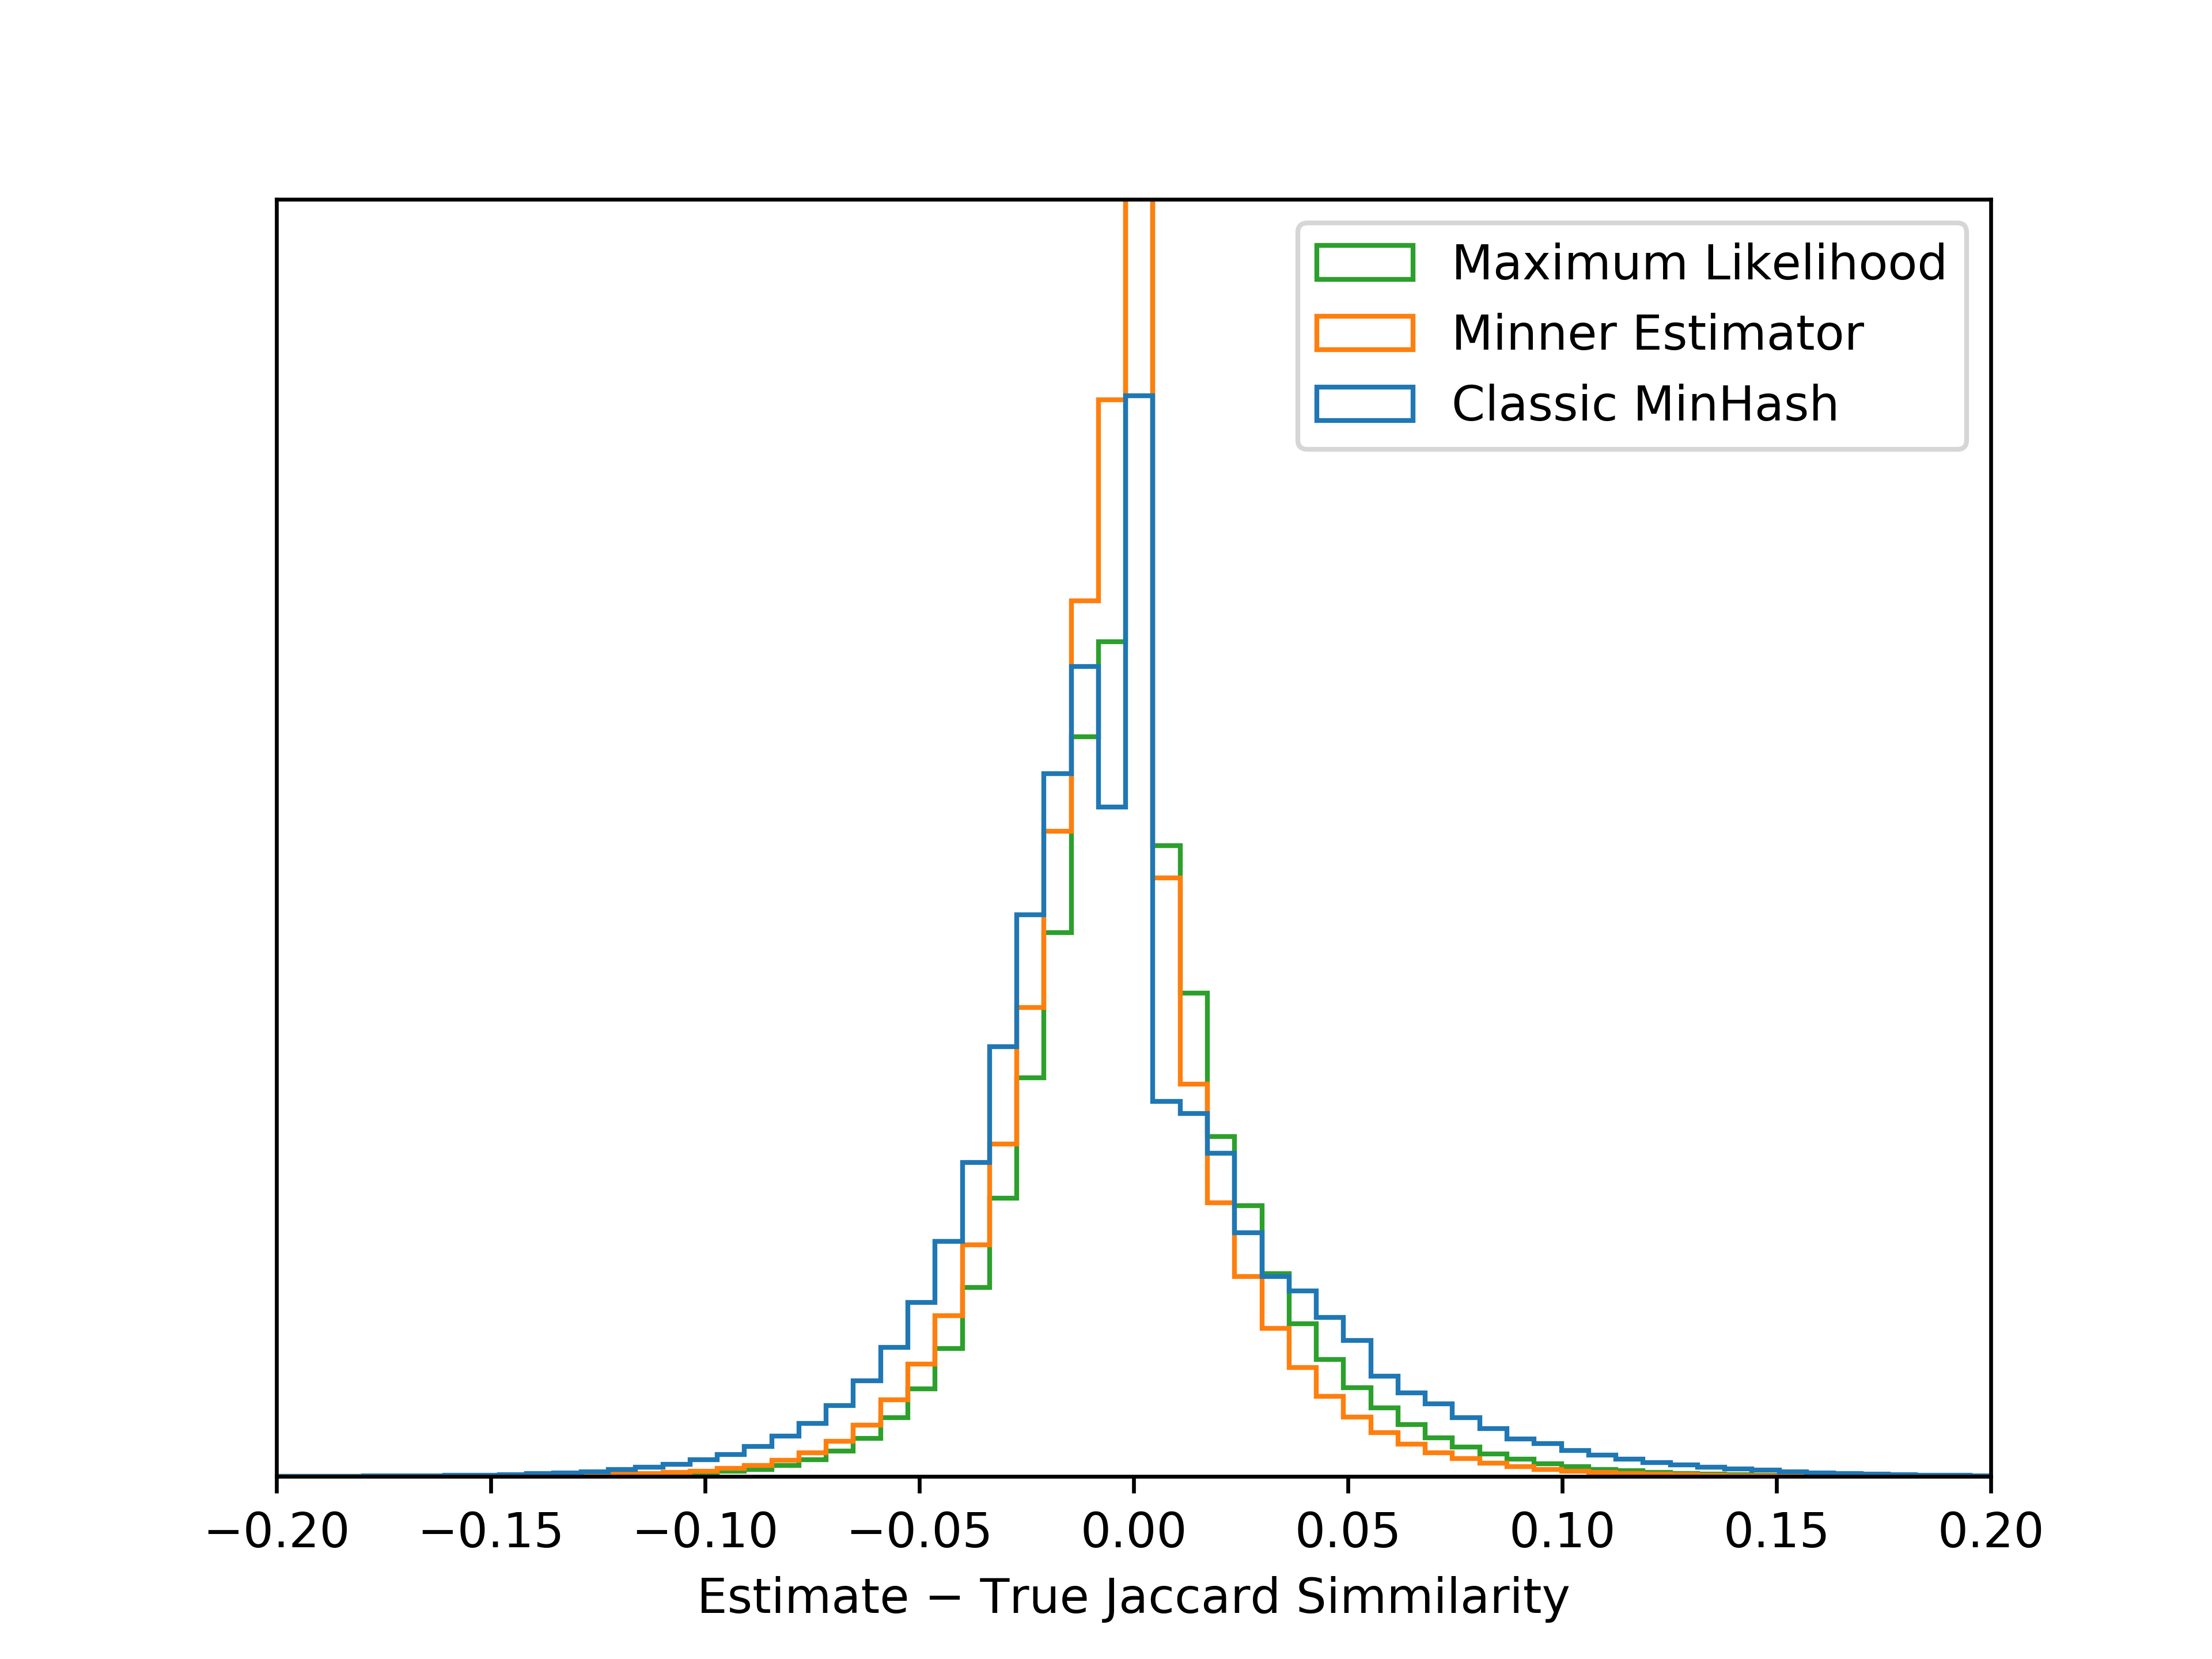
\includegraphics[trim=0 5 35 40,clip,width=\linewidth]{figures/hist2}
\caption{Density of estimation errors on Netflix dataset at $K=31$.
   %The empiric means are $0.0114$ for the symmetric estimator, 
%$0.0002$ for the fast estimator, and 
%$0.0038$ for the MLE estimator.
}
\end{figure}

\begin{figure}
   \centering
   % trim is left bottom right top
   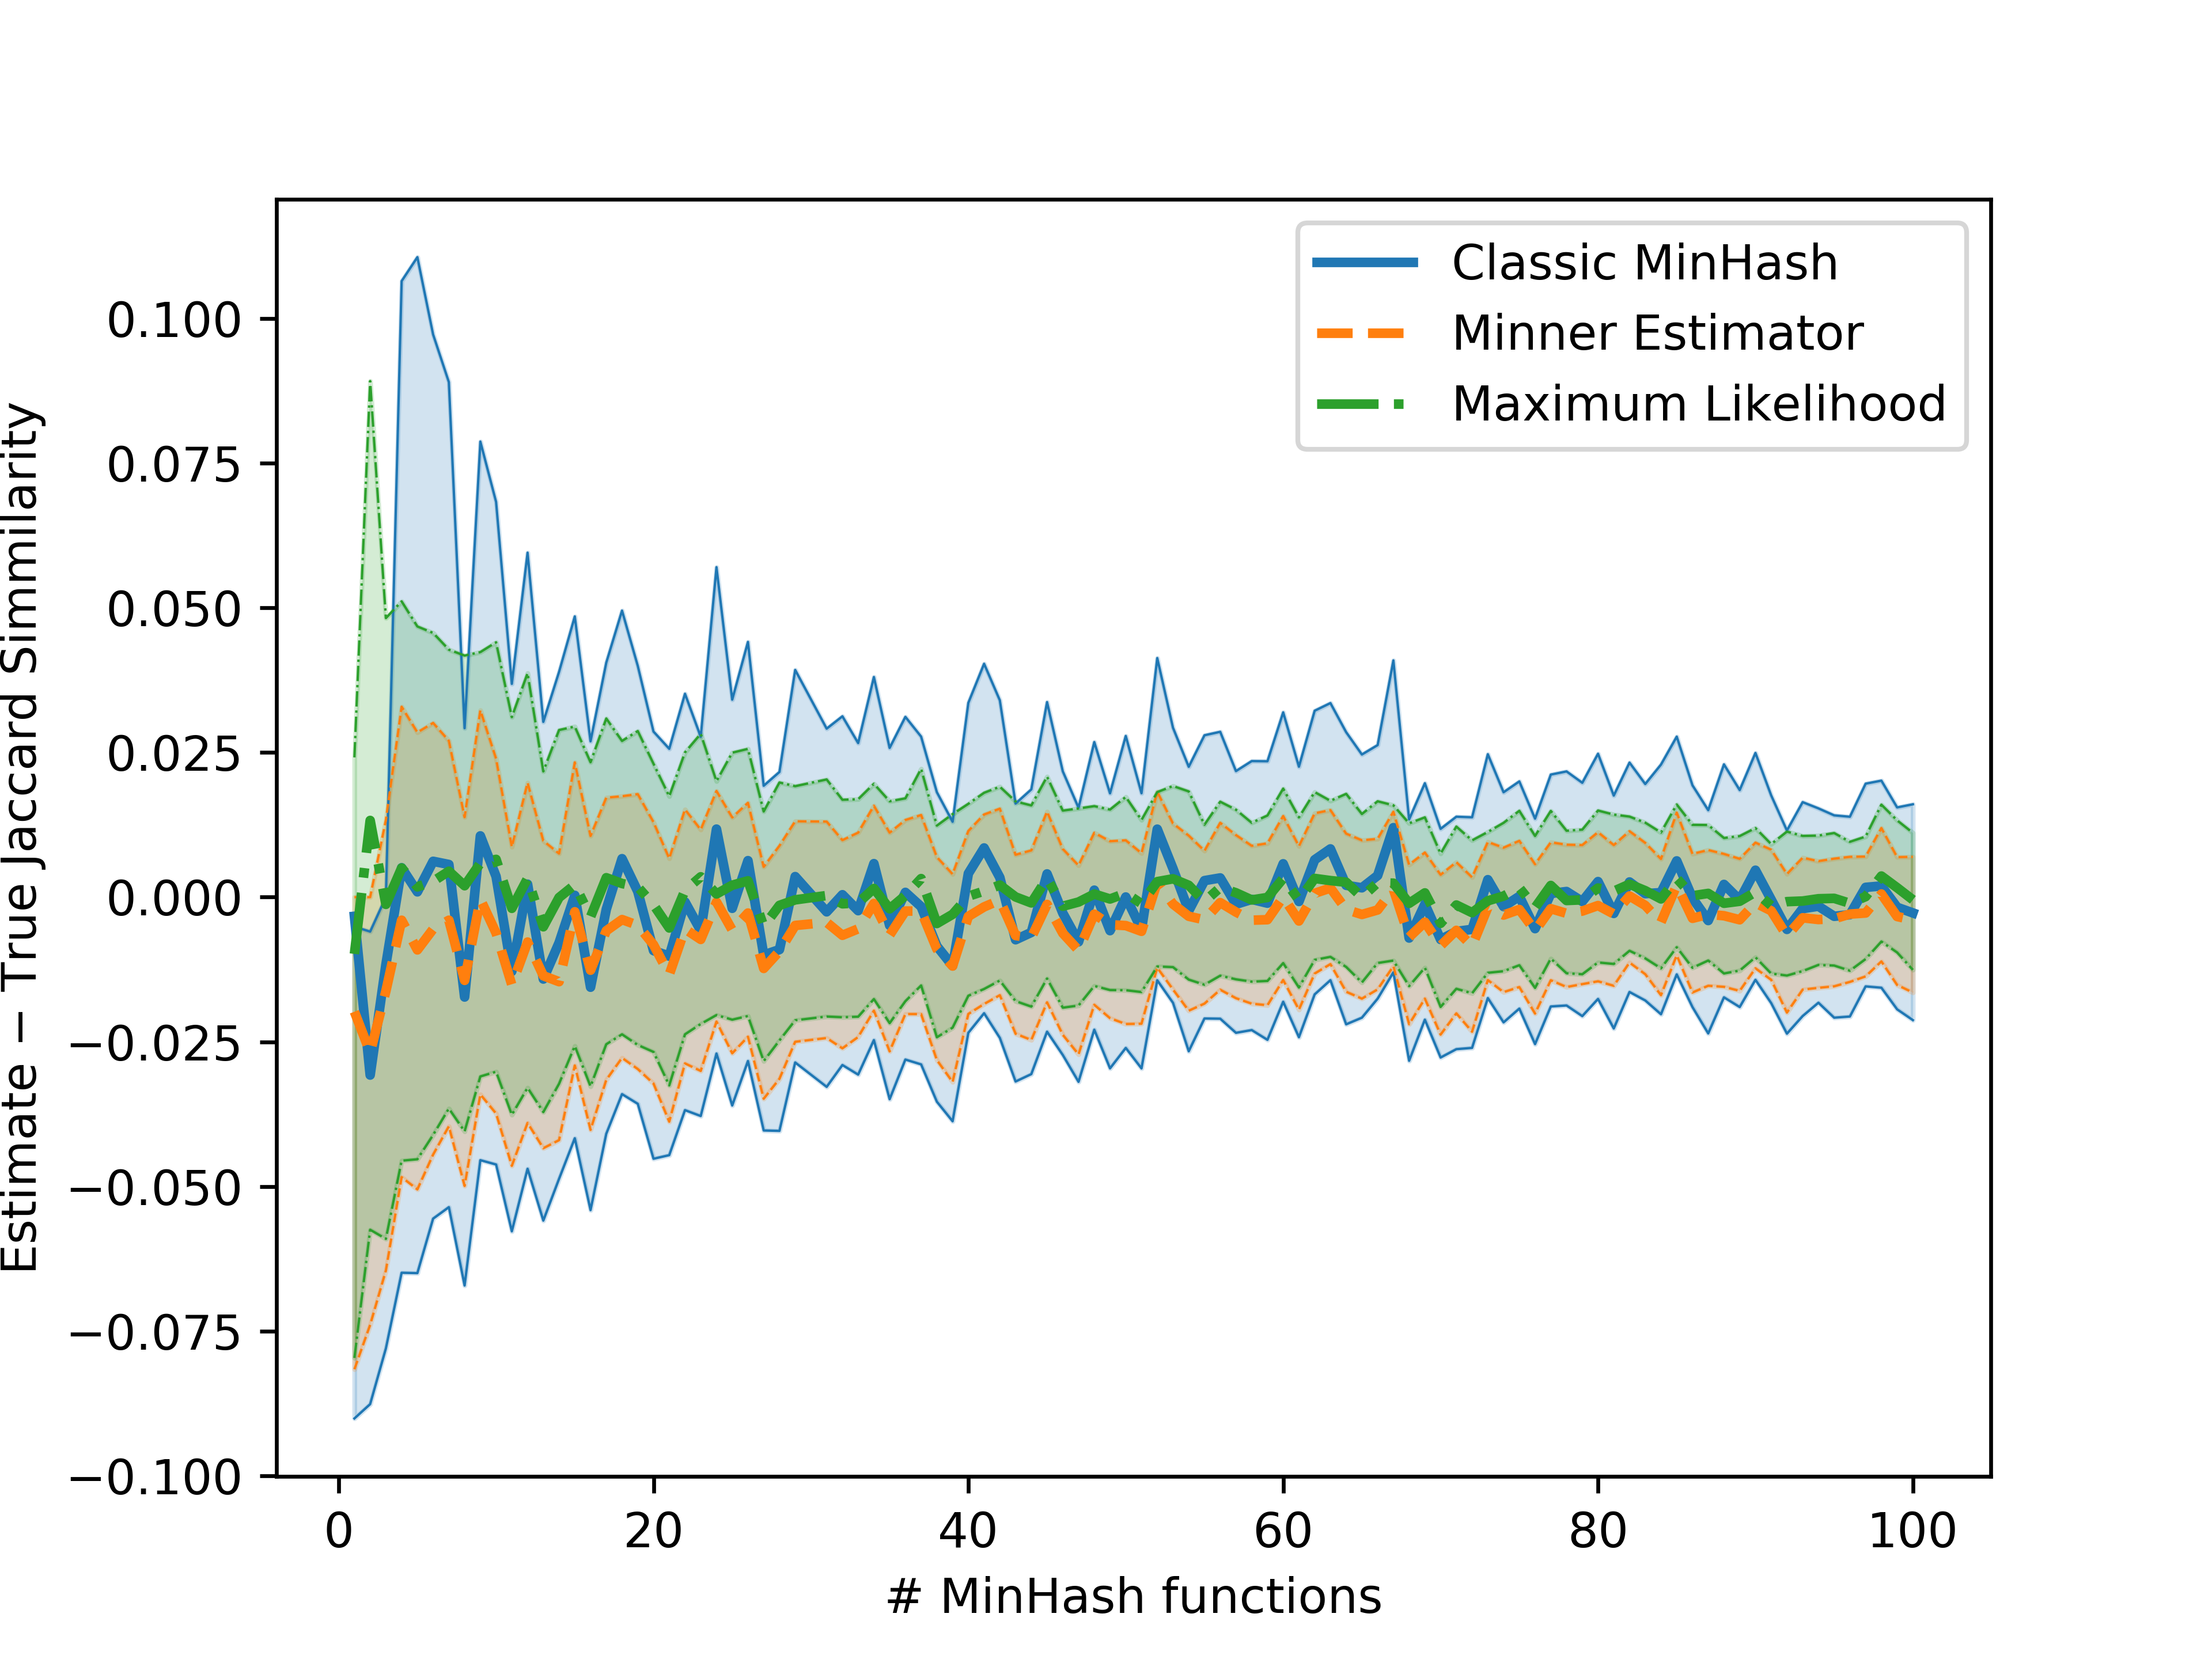
\includegraphics[trim=0 0 35 40,clip,width=\linewidth]{figures/var2}
   \caption{
      Mean values with 1 standard deviation bounds (15.9\% percentile)
      on the estimation error for 5 million pairs from the Netflix dataset.
   }
   \label{fig:var}
\end{figure}
